% Options for packages loaded elsewhere
\PassOptionsToPackage{unicode}{hyperref}
\PassOptionsToPackage{hyphens}{url}
\PassOptionsToPackage{dvipsnames,svgnames,x11names}{xcolor}
%
\documentclass[
  letterpaper,
  DIV=11,
  numbers=noendperiod]{scrartcl}

\usepackage{amsmath,amssymb}
\usepackage{lmodern}
\usepackage{iftex}
\ifPDFTeX
  \usepackage[T1]{fontenc}
  \usepackage[utf8]{inputenc}
  \usepackage{textcomp} % provide euro and other symbols
\else % if luatex or xetex
  \usepackage{unicode-math}
  \defaultfontfeatures{Scale=MatchLowercase}
  \defaultfontfeatures[\rmfamily]{Ligatures=TeX,Scale=1}
\fi
% Use upquote if available, for straight quotes in verbatim environments
\IfFileExists{upquote.sty}{\usepackage{upquote}}{}
\IfFileExists{microtype.sty}{% use microtype if available
  \usepackage[]{microtype}
  \UseMicrotypeSet[protrusion]{basicmath} % disable protrusion for tt fonts
}{}
\makeatletter
\@ifundefined{KOMAClassName}{% if non-KOMA class
  \IfFileExists{parskip.sty}{%
    \usepackage{parskip}
  }{% else
    \setlength{\parindent}{0pt}
    \setlength{\parskip}{6pt plus 2pt minus 1pt}}
}{% if KOMA class
  \KOMAoptions{parskip=half}}
\makeatother
\usepackage{xcolor}
\setlength{\emergencystretch}{3em} % prevent overfull lines
\setcounter{secnumdepth}{-\maxdimen} % remove section numbering
% Make \paragraph and \subparagraph free-standing
\ifx\paragraph\undefined\else
  \let\oldparagraph\paragraph
  \renewcommand{\paragraph}[1]{\oldparagraph{#1}\mbox{}}
\fi
\ifx\subparagraph\undefined\else
  \let\oldsubparagraph\subparagraph
  \renewcommand{\subparagraph}[1]{\oldsubparagraph{#1}\mbox{}}
\fi

\usepackage{color}
\usepackage{fancyvrb}
\newcommand{\VerbBar}{|}
\newcommand{\VERB}{\Verb[commandchars=\\\{\}]}
\DefineVerbatimEnvironment{Highlighting}{Verbatim}{commandchars=\\\{\}}
% Add ',fontsize=\small' for more characters per line
\usepackage{framed}
\definecolor{shadecolor}{RGB}{241,243,245}
\newenvironment{Shaded}{\begin{snugshade}}{\end{snugshade}}
\newcommand{\AlertTok}[1]{\textcolor[rgb]{0.68,0.00,0.00}{#1}}
\newcommand{\AnnotationTok}[1]{\textcolor[rgb]{0.37,0.37,0.37}{#1}}
\newcommand{\AttributeTok}[1]{\textcolor[rgb]{0.40,0.45,0.13}{#1}}
\newcommand{\BaseNTok}[1]{\textcolor[rgb]{0.68,0.00,0.00}{#1}}
\newcommand{\BuiltInTok}[1]{\textcolor[rgb]{0.00,0.23,0.31}{#1}}
\newcommand{\CharTok}[1]{\textcolor[rgb]{0.13,0.47,0.30}{#1}}
\newcommand{\CommentTok}[1]{\textcolor[rgb]{0.37,0.37,0.37}{#1}}
\newcommand{\CommentVarTok}[1]{\textcolor[rgb]{0.37,0.37,0.37}{\textit{#1}}}
\newcommand{\ConstantTok}[1]{\textcolor[rgb]{0.56,0.35,0.01}{#1}}
\newcommand{\ControlFlowTok}[1]{\textcolor[rgb]{0.00,0.23,0.31}{#1}}
\newcommand{\DataTypeTok}[1]{\textcolor[rgb]{0.68,0.00,0.00}{#1}}
\newcommand{\DecValTok}[1]{\textcolor[rgb]{0.68,0.00,0.00}{#1}}
\newcommand{\DocumentationTok}[1]{\textcolor[rgb]{0.37,0.37,0.37}{\textit{#1}}}
\newcommand{\ErrorTok}[1]{\textcolor[rgb]{0.68,0.00,0.00}{#1}}
\newcommand{\ExtensionTok}[1]{\textcolor[rgb]{0.00,0.23,0.31}{#1}}
\newcommand{\FloatTok}[1]{\textcolor[rgb]{0.68,0.00,0.00}{#1}}
\newcommand{\FunctionTok}[1]{\textcolor[rgb]{0.28,0.35,0.67}{#1}}
\newcommand{\ImportTok}[1]{\textcolor[rgb]{0.00,0.46,0.62}{#1}}
\newcommand{\InformationTok}[1]{\textcolor[rgb]{0.37,0.37,0.37}{#1}}
\newcommand{\KeywordTok}[1]{\textcolor[rgb]{0.00,0.23,0.31}{#1}}
\newcommand{\NormalTok}[1]{\textcolor[rgb]{0.00,0.23,0.31}{#1}}
\newcommand{\OperatorTok}[1]{\textcolor[rgb]{0.37,0.37,0.37}{#1}}
\newcommand{\OtherTok}[1]{\textcolor[rgb]{0.00,0.23,0.31}{#1}}
\newcommand{\PreprocessorTok}[1]{\textcolor[rgb]{0.68,0.00,0.00}{#1}}
\newcommand{\RegionMarkerTok}[1]{\textcolor[rgb]{0.00,0.23,0.31}{#1}}
\newcommand{\SpecialCharTok}[1]{\textcolor[rgb]{0.37,0.37,0.37}{#1}}
\newcommand{\SpecialStringTok}[1]{\textcolor[rgb]{0.13,0.47,0.30}{#1}}
\newcommand{\StringTok}[1]{\textcolor[rgb]{0.13,0.47,0.30}{#1}}
\newcommand{\VariableTok}[1]{\textcolor[rgb]{0.07,0.07,0.07}{#1}}
\newcommand{\VerbatimStringTok}[1]{\textcolor[rgb]{0.13,0.47,0.30}{#1}}
\newcommand{\WarningTok}[1]{\textcolor[rgb]{0.37,0.37,0.37}{\textit{#1}}}

\providecommand{\tightlist}{%
  \setlength{\itemsep}{0pt}\setlength{\parskip}{0pt}}\usepackage{longtable,booktabs,array}
\usepackage{calc} % for calculating minipage widths
% Correct order of tables after \paragraph or \subparagraph
\usepackage{etoolbox}
\makeatletter
\patchcmd\longtable{\par}{\if@noskipsec\mbox{}\fi\par}{}{}
\makeatother
% Allow footnotes in longtable head/foot
\IfFileExists{footnotehyper.sty}{\usepackage{footnotehyper}}{\usepackage{footnote}}
\makesavenoteenv{longtable}
\usepackage{graphicx}
\makeatletter
\def\maxwidth{\ifdim\Gin@nat@width>\linewidth\linewidth\else\Gin@nat@width\fi}
\def\maxheight{\ifdim\Gin@nat@height>\textheight\textheight\else\Gin@nat@height\fi}
\makeatother
% Scale images if necessary, so that they will not overflow the page
% margins by default, and it is still possible to overwrite the defaults
% using explicit options in \includegraphics[width, height, ...]{}
\setkeys{Gin}{width=\maxwidth,height=\maxheight,keepaspectratio}
% Set default figure placement to htbp
\makeatletter
\def\fps@figure{htbp}
\makeatother

\KOMAoption{captions}{tableheading}
\makeatletter
\makeatother
\makeatletter
\makeatother
\makeatletter
\@ifpackageloaded{caption}{}{\usepackage{caption}}
\AtBeginDocument{%
\ifdefined\contentsname
  \renewcommand*\contentsname{Table of contents}
\else
  \newcommand\contentsname{Table of contents}
\fi
\ifdefined\listfigurename
  \renewcommand*\listfigurename{List of Figures}
\else
  \newcommand\listfigurename{List of Figures}
\fi
\ifdefined\listtablename
  \renewcommand*\listtablename{List of Tables}
\else
  \newcommand\listtablename{List of Tables}
\fi
\ifdefined\figurename
  \renewcommand*\figurename{Figure}
\else
  \newcommand\figurename{Figure}
\fi
\ifdefined\tablename
  \renewcommand*\tablename{Table}
\else
  \newcommand\tablename{Table}
\fi
}
\@ifpackageloaded{float}{}{\usepackage{float}}
\floatstyle{ruled}
\@ifundefined{c@chapter}{\newfloat{codelisting}{h}{lop}}{\newfloat{codelisting}{h}{lop}[chapter]}
\floatname{codelisting}{Listing}
\newcommand*\listoflistings{\listof{codelisting}{List of Listings}}
\makeatother
\makeatletter
\@ifpackageloaded{caption}{}{\usepackage{caption}}
\@ifpackageloaded{subcaption}{}{\usepackage{subcaption}}
\makeatother
\makeatletter
\@ifpackageloaded{tcolorbox}{}{\usepackage[many]{tcolorbox}}
\makeatother
\makeatletter
\@ifundefined{shadecolor}{\definecolor{shadecolor}{rgb}{.97, .97, .97}}
\makeatother
\makeatletter
\makeatother
\ifLuaTeX
  \usepackage{selnolig}  % disable illegal ligatures
\fi
\IfFileExists{bookmark.sty}{\usepackage{bookmark}}{\usepackage{hyperref}}
\IfFileExists{xurl.sty}{\usepackage{xurl}}{} % add URL line breaks if available
\urlstyle{same} % disable monospaced font for URLs
\hypersetup{
  pdftitle={Internal and external valdity of empirical models},
  pdfauthor={Zahid Asghar   School of Economics, QAU, Islamabad},
  colorlinks=true,
  linkcolor={blue},
  filecolor={Maroon},
  citecolor={Blue},
  urlcolor={Blue},
  pdfcreator={LaTeX via pandoc}}

\title{Internal and external valdity of empirical models}
\author{Zahid Asghar School of Economics, QAU, Islamabad}
\date{}

\begin{document}
\maketitle
\ifdefined\Shaded\renewenvironment{Shaded}{\begin{tcolorbox}[interior hidden, frame hidden, sharp corners, breakable, enhanced, boxrule=0pt, borderline west={3pt}{0pt}{shadecolor}]}{\end{tcolorbox}}\fi

\hypertarget{internal-validity-of-regression-studies}{%
\section{Internal validity of regression
studies}\label{internal-validity-of-regression-studies}}

\hypertarget{goal-of-this-study}{%
\subsection{Goal of this study}\label{goal-of-this-study}}

\begin{itemize}
\tightlist
\item
  Internal versus External Validity
\item
  Testing for Heteroskedasticity
\end{itemize}

\begin{quote}
A statistical analysis has internal validity if the statistical
inference made about causal effects are valid for the considered
population.
\end{quote}

\begin{quote}
An analysis is said to have external validity if inferences and
conclusion are valid for the studies' population and can be generalized
to other populations and settings.
\end{quote}

\hypertarget{internal-and-external-validity-of-regression}{%
\subsection{Internal and External Validity of
Regression}\label{internal-and-external-validity-of-regression}}

\begin{itemize}
\tightlist
\item
  Internal validity is satisfied if the statistical inference about the
  causal effects are valid for the population being studied.
\item
  External validity would need the inferences and conclusions to be
  generalized from the population and setting studied to other
  populations and setting.
\item
  Example: Think about the california test example.
\item
  Is the slope, βstr , unbiased and consistent?
\item
  Is this a valid estimate for NY?, WV?, NM?,. . .
\end{itemize}

\hypertarget{threats-to-internal-validity}{%
\subsection{Threats to internal
validity}\label{threats-to-internal-validity}}

\begin{enumerate}
\def\labelenumi{\arabic{enumi}.}
\tightlist
\item
  Omitted Variable Bias
\item
  Misspecification of Functional Form of Regression Model
\item
  Measurement Error
\item
  Missing Data and Sample Selection
\item
  Simultaneous Causality In each case, OLS assumption \(#1\) is
  violated: \(E(u_i| X_{1i}, X_{2i}, \dots,X_{ki})\neq 0.\)
\end{enumerate}

\hypertarget{omitted-variable-bias}{%
\subsection{Omitted variable bias}\label{omitted-variable-bias}}

\begin{itemize}
\tightlist
\item
  If you have the data for omitted variables:

  \begin{itemize}
  \tightlist
  \item
    Be specific about your coefficient of interest.
  \item
    Use a priori reason for adding variables.
  \item
    Use statistical tests for questionable variables (t and F).
  \item
    Provide all the potential specifications in tabular form.
  \end{itemize}
\item
  What if you don't have the data:

  \begin{itemize}
  \tightlist
  \item
    Panel data (next chapter)
  \item
    IV method (chapter 12)
  \item
    Randomized control experiments
  \end{itemize}
\end{itemize}

\hypertarget{misspecification-of-functional-form-of-regression-model}{%
\subsection{Misspecification of Functional Form of Regression
Model}\label{misspecification-of-functional-form-of-regression-model}}

\begin{itemize}
\tightlist
\item
  For continuous dependent variable: Use methods discussed in chapter 8
  to modify functional forms.
\item
  For discrete or binary dependent variable: Chapter 11 (we will get
  there. . . ).
\end{itemize}

\hypertarget{section}{%
\subsection{}\label{section}}

Lets our model is \(Y_i = X_i^2\) but one uses
\(Y_i=\beta_0+\beta_1X_{1i}+u_i\)

\hypertarget{code}{%
\paragraph{Code}\label{code}}

\begin{Shaded}
\begin{Highlighting}[]
\CommentTok{\# set seed for reproducibility}
\FunctionTok{set.seed}\NormalTok{(}\DecValTok{5}\NormalTok{)}
\FunctionTok{library}\NormalTok{(tidyverse)}
\end{Highlighting}
\end{Shaded}

\begin{verbatim}
-- Attaching packages --------------------------------------- tidyverse 1.3.2 --
v ggplot2 3.3.6     v purrr   0.3.4
v tibble  3.1.7     v dplyr   1.0.9
v tidyr   1.2.0     v stringr 1.4.0
v readr   2.1.2     v forcats 0.5.1
-- Conflicts ------------------------------------------ tidyverse_conflicts() --
x dplyr::filter() masks stats::filter()
x dplyr::lag()    masks stats::lag()
\end{verbatim}

\begin{Shaded}
\begin{Highlighting}[]
\CommentTok{\# simulate data set}
\NormalTok{X }\OtherTok{\textless{}{-}} \FunctionTok{runif}\NormalTok{(}\DecValTok{100}\NormalTok{, }\SpecialCharTok{{-}}\DecValTok{5}\NormalTok{, }\DecValTok{5}\NormalTok{)}
\NormalTok{Y }\OtherTok{\textless{}{-}}\NormalTok{ X}\SpecialCharTok{\^{}}\DecValTok{2} \SpecialCharTok{+} \FunctionTok{rnorm}\NormalTok{(}\DecValTok{100}\NormalTok{)}
\NormalTok{df}\OtherTok{\textless{}{-}}\FunctionTok{cbind}\NormalTok{(X,Y)}
\NormalTok{df}\OtherTok{\textless{}{-}}\FunctionTok{as.data.frame}\NormalTok{(df)}
\end{Highlighting}
\end{Shaded}

\hypertarget{output}{%
\paragraph{Output}\label{output}}

\begin{Shaded}
\begin{Highlighting}[]
\CommentTok{\# estimate the regression function}
\NormalTok{ms\_mod }\OtherTok{\textless{}{-}} \FunctionTok{lm}\NormalTok{(Y }\SpecialCharTok{\textasciitilde{}}\NormalTok{ X)}
\NormalTok{ms\_mod}
\end{Highlighting}
\end{Shaded}

\begin{Shaded}
\begin{Highlighting}[]
\CommentTok{\# set seed for reproducibility}
\FunctionTok{set.seed}\NormalTok{(}\DecValTok{5}\NormalTok{)}
\FunctionTok{library}\NormalTok{(tidyverse)}
\CommentTok{\# simulate data set}
\NormalTok{X }\OtherTok{\textless{}{-}} \FunctionTok{runif}\NormalTok{(}\DecValTok{100}\NormalTok{, }\SpecialCharTok{{-}}\DecValTok{5}\NormalTok{, }\DecValTok{5}\NormalTok{)}
\NormalTok{Y }\OtherTok{\textless{}{-}}\NormalTok{ X}\SpecialCharTok{\^{}}\DecValTok{2} \SpecialCharTok{+} \FunctionTok{rnorm}\NormalTok{(}\DecValTok{100}\NormalTok{)}
\NormalTok{df}\OtherTok{\textless{}{-}}\FunctionTok{cbind}\NormalTok{(X,Y)}
\NormalTok{df}\OtherTok{\textless{}{-}}\FunctionTok{as.data.frame}\NormalTok{(df)}
\CommentTok{\# estimate the regression function}
\NormalTok{ms\_mod }\OtherTok{\textless{}{-}} \FunctionTok{lm}\NormalTok{(Y }\SpecialCharTok{\textasciitilde{}}\NormalTok{ X)}
\NormalTok{ms\_mod}
\end{Highlighting}
\end{Shaded}

\begin{verbatim}

Call:
lm(formula = Y ~ X)

Coefficients:
(Intercept)            X  
     9.0173       0.4353  
\end{verbatim}

\hypertarget{plot-this-linear-fit}{%
\subsection{Plot this linear fit}\label{plot-this-linear-fit}}

\begin{Shaded}
\begin{Highlighting}[]
\FunctionTok{ggplot}\NormalTok{(df)}\SpecialCharTok{+}\FunctionTok{aes}\NormalTok{(X,Y)}\SpecialCharTok{+}\FunctionTok{geom\_point}\NormalTok{()}\SpecialCharTok{+}\FunctionTok{geom\_smooth}\NormalTok{(}\AttributeTok{method =} \StringTok{"lm"}\NormalTok{,}\AttributeTok{se=}\ConstantTok{FALSE}\NormalTok{)}
\end{Highlighting}
\end{Shaded}

\begin{verbatim}
`geom_smooth()` using formula 'y ~ x'
\end{verbatim}

\begin{figure}[H]

{\centering 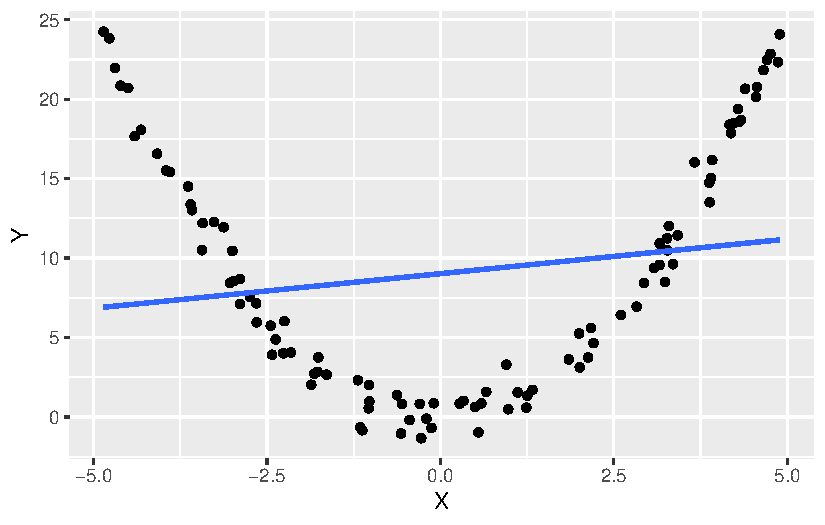
\includegraphics{assesing_regression_files/figure-pdf/unnamed-chunk-4-1.pdf}

}

\end{figure}

\hypertarget{measurement-error-in-x}{%
\subsection{\texorpdfstring{Measurement Error in
\(X\)}{Measurement Error in X}}\label{measurement-error-in-x}}

General regression model: \(Y_i = \beta_0 + \beta_1X_{i} + u_{i}\) What
you would like to measure is \(X_i\), but what you do actually measure
is \(\overset{\sim}{X}_i\). Then the error is
\(X_i - \overset{\sim}{X}_i\)

\begin{itemize}
\tightlist
\item
  Regression model with mesurement error \(\overset{\sim}{X}_i\) instead
  of \(X_i\)
  \(\begin{align*} Y_i =& \, \beta_0 + \beta_1 \overset{\sim}{X}_i + \underbrace{\beta_1 (X_i - \overset{\sim}{X}_i) + u_i}_{=v_i} \\ Y_i =& \, \beta_0 + \beta_1 \overset{\sim}{X}_i + v_i \end{align*}\)
\end{itemize}

Rewrite \(ν_i = \beta_1 (X_i - \overset{\sim}{X}_i)+u_i\)

\hypertarget{section-1}{%
\subsection{}\label{section-1}}

\[\begin{align*}
  Y_i =& \, \beta_0 + \beta_1 \overset{\sim}{X}_i + \underbrace{\beta_1 (X_i - \overset{\sim}{X}_i) + u_i}_{=v_i} \\
  Y_i =& \, \beta_0 + \beta_1 \overset{\sim}{X}_i + v_i
\end{align*}\]

where here \(\overset{\sim}{X}_i\) and \(v_i\) are correlated resulting
to slope coefficient \(\hat{\beta_1}\) to be biased.

\hypertarget{section-2}{%
\subsection{}\label{section-2}}

The classical measurement error model assumes that the measurement
error, \(w_i\), has zero mean and that it is uncorrelated with the
variable, \(\overset{\sim}{X}_i\), and the error term of the population
regression model, \(u_i\):
\(\begin{equation} \overset{\sim}{X}_i = X_i + w_i, \ \ \rho_{w_i,u_i}=0, \ \ \rho_{w_i,X_i}=0 \end{equation}\)
This holds
\(\begin{equation} \widehat{\beta}_1 \xrightarrow{p}{\frac{\sigma_{X}^2}{\sigma_{X}^2 + \sigma_{w}^2}} \beta_1 \tag{9.1} \end{equation}\)

\hypertarget{section-3}{%
\subsection{}\label{section-3}}

\(\sigma_{X}^2, \sigma_{w}^2 > 0\) so \(\hat{\beta_1}\) smaller than 1.

\begin{enumerate}
\def\labelenumi{\arabic{enumi}.}
\item
  If there is no measurement error, \(\sigma_{w}^2=0\) such that
  \(\widehat{\beta}_1 \xrightarrow{p}{\beta_1}\) .
\item
  If \(\sigma_{w}^2 \gg \sigma_{X}^2\) we have
  \(\widehat{\beta}_1 \xrightarrow{p}{0}\)
\end{enumerate}

This is the case if the measurement error is so large that there
essentially is no information on \(X\) in the data that can be used to
estimate \(\beta\).

\hypertarget{section-4}{%
\subsection{}\label{section-4}}

\(\begin{align} (X, Y) \sim \mathcal{N}\left[\begin{pmatrix}50\\ 100\end{pmatrix},\begin{pmatrix}10 & 5 \\ 5 & 10 \end{pmatrix}\right] \tag{9.3} \end{align}\)

\(\begin{align*} Y_i =& \, 100 + 0.5 (X_i - 50) \\ =& \, 75 + 0.5 X_i. \tag{9.4} \end{align*}\)

\(\overset{\sim}{X_i} = X_i + w_i\)
\(w_i \overset{i.i.d.}{\sim} \mathcal{N}(0,10)\) \(w_i\) is independent
of \(x_i\).

\hypertarget{section-5}{%
\subsection{}\label{section-5}}

\begin{Shaded}
\begin{Highlighting}[]
\CommentTok{\# set seed}
\FunctionTok{set.seed}\NormalTok{(}\DecValTok{1}\NormalTok{)}

\CommentTok{\# load the package \textquotesingle{}mvtnorm\textquotesingle{} and simulate bivariate normal data}
\FunctionTok{library}\NormalTok{(mvtnorm)}
\NormalTok{dat }\OtherTok{\textless{}{-}} \FunctionTok{data.frame}\NormalTok{(}
  \FunctionTok{rmvnorm}\NormalTok{(}\DecValTok{1000}\NormalTok{, }\FunctionTok{c}\NormalTok{(}\DecValTok{50}\NormalTok{, }\DecValTok{100}\NormalTok{), }
          \AttributeTok{sigma =} \FunctionTok{cbind}\NormalTok{(}\FunctionTok{c}\NormalTok{(}\DecValTok{10}\NormalTok{, }\DecValTok{5}\NormalTok{), }\FunctionTok{c}\NormalTok{(}\DecValTok{5}\NormalTok{, }\DecValTok{10}\NormalTok{))))}

\CommentTok{\# set columns names}
\FunctionTok{colnames}\NormalTok{(dat) }\OtherTok{\textless{}{-}} \FunctionTok{c}\NormalTok{(}\StringTok{"X"}\NormalTok{, }\StringTok{"Y"}\NormalTok{)}
\end{Highlighting}
\end{Shaded}

\hypertarget{section-6}{%
\subsection{}\label{section-6}}

\begin{Shaded}
\begin{Highlighting}[]
\CommentTok{\# estimate the model (without measurement error)}
\NormalTok{noerror\_mod }\OtherTok{\textless{}{-}} \FunctionTok{lm}\NormalTok{(Y }\SpecialCharTok{\textasciitilde{}}\NormalTok{ X, }\AttributeTok{data =}\NormalTok{ dat)}

\CommentTok{\# estimate the model (with measurement error in X)}
\NormalTok{dat}\SpecialCharTok{$}\NormalTok{X }\OtherTok{\textless{}{-}}\NormalTok{ dat}\SpecialCharTok{$}\NormalTok{X }\SpecialCharTok{+} \FunctionTok{rnorm}\NormalTok{(}\AttributeTok{n =} \DecValTok{1000}\NormalTok{, }\AttributeTok{sd =} \FunctionTok{sqrt}\NormalTok{(}\DecValTok{10}\NormalTok{))}
\NormalTok{error\_mod }\OtherTok{\textless{}{-}} \FunctionTok{lm}\NormalTok{(Y }\SpecialCharTok{\textasciitilde{}}\NormalTok{ X, }\AttributeTok{data =}\NormalTok{ dat)}

\CommentTok{\# print estimated coefficients to console}
\NormalTok{noerror\_mod}\SpecialCharTok{$}\NormalTok{coefficients}
\end{Highlighting}
\end{Shaded}

\begin{verbatim}
(Intercept)           X 
 76.3002047   0.4755264 
\end{verbatim}

\begin{Shaded}
\begin{Highlighting}[]
\NormalTok{error\_mod}\SpecialCharTok{$}\NormalTok{coefficients}
\end{Highlighting}
\end{Shaded}

\begin{verbatim}
(Intercept)           X 
  87.276004    0.255212 
\end{verbatim}

\hypertarget{plots}{%
\subsection{Plots}\label{plots}}

\begin{Shaded}
\begin{Highlighting}[]
\CommentTok{\# plot sample data}
\FunctionTok{plot}\NormalTok{(dat}\SpecialCharTok{$}\NormalTok{X, dat}\SpecialCharTok{$}\NormalTok{Y, }
     \AttributeTok{pch =} \DecValTok{20}\NormalTok{, }
     \AttributeTok{col =} \StringTok{"steelblue"}\NormalTok{,}
     \AttributeTok{xlab =} \StringTok{"X"}\NormalTok{,}
     \AttributeTok{ylab =} \StringTok{"Y"}\NormalTok{)}

\CommentTok{\# add population regression function}
\FunctionTok{abline}\NormalTok{(}\AttributeTok{coef =} \FunctionTok{c}\NormalTok{(}\DecValTok{75}\NormalTok{, }\FloatTok{0.5}\NormalTok{), }
       \AttributeTok{col =} \StringTok{"darkgreen"}\NormalTok{,}
       \AttributeTok{lwd  =} \FloatTok{1.5}\NormalTok{)}

\CommentTok{\# add estimated regression functions}
\FunctionTok{abline}\NormalTok{(noerror\_mod, }
       \AttributeTok{col =} \StringTok{"purple"}\NormalTok{,}
       \AttributeTok{lwd  =} \FloatTok{1.5}\NormalTok{)}

\FunctionTok{abline}\NormalTok{(error\_mod, }
       \AttributeTok{col =} \StringTok{"darkred"}\NormalTok{,}
       \AttributeTok{lwd  =} \FloatTok{1.5}\NormalTok{)}

\CommentTok{\# add legend}
\FunctionTok{legend}\NormalTok{(}\StringTok{"topleft"}\NormalTok{,}
       \AttributeTok{bg =} \StringTok{"transparent"}\NormalTok{,}
       \AttributeTok{cex =} \FloatTok{0.8}\NormalTok{,}
       \AttributeTok{lty =} \DecValTok{1}\NormalTok{,}
       \AttributeTok{col =} \FunctionTok{c}\NormalTok{(}\StringTok{"darkgreen"}\NormalTok{, }\StringTok{"purple"}\NormalTok{, }\StringTok{"darkred"}\NormalTok{), }
       \AttributeTok{legend =} \FunctionTok{c}\NormalTok{(}\StringTok{"Population"}\NormalTok{, }\StringTok{"No Errors"}\NormalTok{, }\StringTok{"Errors"}\NormalTok{))}
\end{Highlighting}
\end{Shaded}

\begin{figure}[H]

{\centering 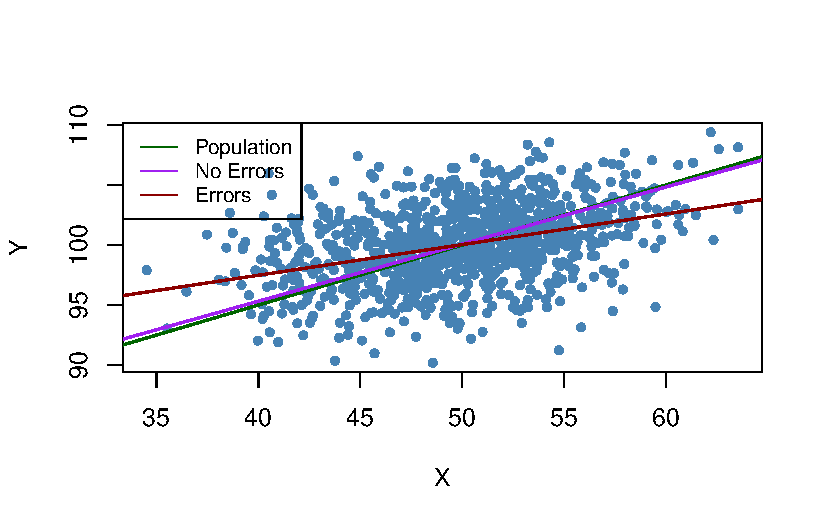
\includegraphics{assesing_regression_files/figure-pdf/unnamed-chunk-7-1.pdf}

}

\end{figure}

\hypertarget{plot-in-ggplot}{%
\subsection{plot in ggplot}\label{plot-in-ggplot}}

\begin{Shaded}
\begin{Highlighting}[]
\FunctionTok{ggplot}\NormalTok{(dat)}\SpecialCharTok{+}\FunctionTok{aes}\NormalTok{(X,Y)}\SpecialCharTok{+}\FunctionTok{geom\_point}\NormalTok{()}\SpecialCharTok{+}\FunctionTok{geom\_abline}\NormalTok{()}
\end{Highlighting}
\end{Shaded}

\begin{figure}[H]

{\centering 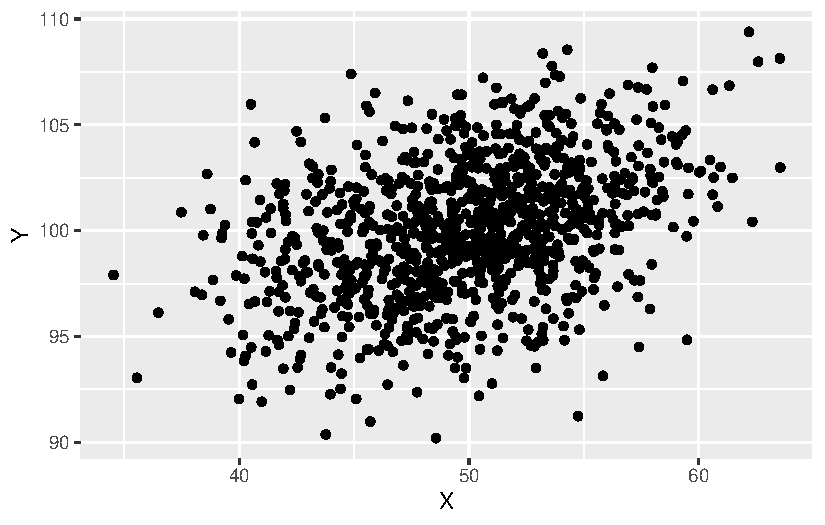
\includegraphics{assesing_regression_files/figure-pdf/unnamed-chunk-8-1.pdf}

}

\end{figure}

\hypertarget{missing-data-and-sample-selection}{%
\subsection{Missing Data and Sample
Selection}\label{missing-data-and-sample-selection}}

\begin{enumerate}
\def\labelenumi{\arabic{enumi}.}
\tightlist
\item
  Missing at random: There is no bias, but it reduces our sample size.
\item
  Missing regressor values: Same as above.
\item
  Missing \(Y\) due to selection process (sample selection bias): For
  example of this type of bias, think about why older, say, baseball
  players are on average better than younger ones.
\end{enumerate}

\hypertarget{sample-selection-bias}{%
\subsection{4. Sample Selection Bias}\label{sample-selection-bias}}

\hypertarget{simultaneous-causality}{%
\subsection{5. Simultaneous Causality}\label{simultaneous-causality}}

Simultaneous Causality Bias So far we have assumed that the changes in
the independent variable \(X\) are responsible for changes in the
dependent variable \(Y\) . When the reverse is also true, we say that
there is simultaneous causality between \(X\) and \(Y\) . This reverse
causality leads to correlation between \(X\) and the error in the
population regression of interest such that the coefficient on \(X\) is
estimated with bias.

\hypertarget{threats-to-internal-validity-of-a-regression-study}{%
\subsection{Threats to Internal Validity of a Regression
Study}\label{threats-to-internal-validity-of-a-regression-study}}

The five primary threats to internal validity of a multiple regression
study are:

\begin{itemize}
\item
  Omitted variables
\item
  Misspecification of functional form
\item
  Errors in variables (measurement errors in the regressors)
\item
  Sample selection
\item
  Simultaneous causality
\end{itemize}

All these threats lead to failure of the first least squares assumption
\(E(u_i\vert X_{1i},\dots ,X_{ki}) \neq 0\)

so that the OLS estimator is biased and inconsistent.

Furthermore, if one does not adjust for heteroskedasticity and/or serial
correlation, incorrect standard errors may be a threat to internal
validity of the study.



\end{document}
